\documentclass[12pt]{article}
\usepackage[top=1in,bottom=1in,left=1in,right=1in]{geometry}
\usepackage{amsfonts} 
\usepackage{alltt}
\usepackage{array}	
\usepackage{graphicx}
\usepackage{tabularx}
\usepackage{verbatim}
\usepackage{setspace}
\usepackage{listings}
\usepackage{amssymb,amsmath, amsthm}

\title{SOEN331: Introduction to Formal Methods\\for Software Engineering\\
Assignment 2 on Extended Finite State Machines}
\author{\begin{tabular}{c}
Alec Adub (40032876) \tabularnewline
Alex Frappier Lachapelle (40019133) \tabularnewline
Robert Nittolo (40032587) \tabularnewline
Pierre-Olivier Trottier (40059235) \tabularnewline\\
\end{tabular}
}
\date{\today}

\begin{document}
\begin{spacing}{1.5}

\maketitle

\newpage

\section{Formal specification}

\noindent \textbf{Autonomous car}

\noindent The EFSM of the autonomous car is the tuple $S = (Q, \Sigma_1, \Sigma_2, q_0, V, \Lambda)$, where\\

\noindent $Q = \{idle, parked~mode, manual~ driving~mode, cruise~mode, panic~mode\}$\\
\noindent $\Sigma_1 = \{ignition, cruise, drive, switch~to~manual, turn~OFF~panic, unforseen~event, turn~OFF\}$\\
\noindent $\Sigma_2 = \{beep, car~is~stopped,  hazard~signal~is~turned~ON, hazard~signal~is~turned~OFF\}$\\
\noindent $q_0: idle$\\
\noindent $V: destination = \{is~set, is~not~ set\}~engine = \{is~idle, is~not~idle\}$\\
\noindent $\Lambda$: Transition specifications\\
\indent 1. $\rightarrow idle$\\
\indent 2. $parked~mode \xrightarrow {\text { cruise~[destination~is~set]}} cruise~mode$\\
\indent 3. $parked~mode \xrightarrow {\text { cruise~[destination~is~not~set]}} manual~driving~mode$\\
\indent 4. $parked~mode \xrightarrow {\text { drive~[engine~is~idle]}} manual~driving~mode$\\
\indent 5. $cruise~mode \xrightarrow {\text { drive~[engine~is~idle]}} parked~mode$\\
\indent 6. $cruise~mode \xrightarrow {\text { unforseen~event/car~is~stopped;~hazard~signal~is~turned~ON}} panic~mode$\\
\indent 7. $cruise~mode \xrightarrow {\text { switch~to~manual}} manual~mode$\\
\indent 8. $manual~driving~mode \rightarrow  parked~mode$\\
\indent 9. $parked~mode \rightarrow   turned~OFF$\\

\newpage
\noindent \textbf{Parked mode}

\noindent The EFSM of the parked is the tuple $S = (Q, \Sigma_1, \Sigma_2, q_0, V, \Lambda)$, where\\

\noindent $Q = \{parked~mode\}$\\
\noindent $\Sigma_1 = \{set~destination\}$\\
\noindent $\Sigma_2 = \{the~navigations~system's~destination~is~set\}$\\
\noindent $q_0: parked$\\
\noindent $\Lambda$: Transition specifications\\
\indent 1. $\rightarrow parked$\\
\indent 2. $parked \xrightarrow {\text { set~destination/the~navigations~system's~destination~is~set}} parked$\\

\newpage
\noindent \textbf{Manual driving mode}

\noindent The EFSM of the manual driving mode is the tuple $S = (Q, \Sigma_1, \Sigma_2, q_0, V, \Lambda)$, where\\

\noindent $Q = \{driving~mode, break~mode\}$\\
\noindent $\Sigma_1 = \{accelerate,reduce~speed,break\}$\\
\noindent $\Sigma_2 = \{engine~runs~faster,engine~is~stopped,
engine~runs~slower\}$\\
\noindent $q_0: driving~mode$\\
\noindent $V: speed:Z~max:Z$\\
\noindent $\Lambda$: Transition specifications\\
\indent 1. $\rightarrow driving~mode$\\
\indent 2. $driving~mode \xrightarrow {\text { accelerate~[speed<max]/engine~runs~faster}} driving~mode$\\
\indent 3. $driving~mode \xrightarrow {\text { reduce~speed~[speed>0]/engine~runs~slower}} driving~mode$\\
\indent 4. $driving~mode \xrightarrow {\text { break/engine~is~stopped}} break~mode$\\
\indent 5. $break~mode \xrightarrow {\text { accelerate/engine~runs~faster}} driving~mode$\\
\newpage
\noindent \textbf{Avoiding obstacles}

\noindent The EFSM of the avoiding obstacles $S = (Q, \Sigma_1, \Sigma_2, q_0, V, \Lambda)$, where\\

\noindent $Q = \{crusing,tailing~mode,change~lane\}$\\
\noindent $\Sigma_1 = \{check~distance,lane~change,check~lane~change\}$\\
\noindent $\Sigma_2 = \{maintain~speed,slow~down\}$\\
\noindent $q_0: crusing$\\
\noindent $V: Distance:Z~threshold~limit:Z$\\
\noindent $\Lambda$: Transition specifications\\
\indent 1. $\rightarrow cruising$\\
\indent 2. $cruising \xrightarrow {\text { check~distance[distance>thresholdLimit]/maintain~speed}} cruising$\\
\indent 3. $cruising \xrightarrow {\text { lane~change/change~one~left~lane}} change~lane$\\
\indent 4. $crusing \xrightarrow {\text { check~distance[distance<thresholdLimit]/slow~down}} tailing~mode$\\
\indent 5. $driving~mode \xrightarrow {\text { break/engine~is~stopped}} break~mode$\\
\indent 6. $tailing~mode \xrightarrow {\text { check~distance[distance<thresholdLimit]/maintain~speed}} crusing$\\

\newpage
\noindent \textbf{Maintain Desired speed}

\noindent The EFSM of maintain desired speed $S = (Q, \Sigma_1, \Sigma_2, q_0, V, \Lambda)$, where\\

\noindent $Q = \{crusing,accelerate,decelerate\}$\\
\noindent $\Sigma_1 = \{check~speed,accelerate~signal\}$\\
\noindent $\Sigma_2 = \{maintain~speed,accelerate,decelerate\}$\\
\noindent $q_0: crusing$\\
\noindent $V: currentSpeed:Z~maxSpeed:Z$\\
\noindent $\Lambda$: Transition specifications\\
\indent 1. $\rightarrow cruising$\\
\indent 2. $cruising \xrightarrow {\text { check~speed[0.95 default < currentSpeed < 1.05 default]/maintain}} cruising$\\
\indent 3. $cruising \xrightarrow {\text { check~speed[currentSpeed<maxSpeed]/decelerate}} accelerate$\\
\indent 4. $cruising \xrightarrow {\text { check~speed[currentSpeed>maxSpeed]/decelerate}} decelerate$\\
\indent 5. $accelerate \xrightarrow {\text { check~speed[0.95 default < currentSpeed < 1.05 default]/maintain}} cruising$\\
\indent 6. $decelerate \xrightarrow {\text { check~speed[0.95 default < currentSpeed < 1.05 default]/maintain}} cruising$\\

\newpage
\noindent \textbf{Panic state}

\noindent The EFSM of the panic state $S = (Q, \Sigma_1, \Sigma_2, q_0, V, \Lambda)$, where\\

\noindent $Q = \{Initial~state,panic,parked\}$\\
\noindent $\Sigma_1 = \{manual~signal~on,automatic~signal~on,check~panic~signal\}$\\
\noindent $\Sigma_2 = \{Stop~and~hazards~ON,panic~signal~OFF\}$\\
\noindent $q_0: initial~state$\\
\noindent $V: UserTurnedSignalPanicSignal = \{ON, OFF\}$\\
\noindent $\Lambda$: Transition specifications\\
\indent 1. $\rightarrow initial~state$\\
\indent 2. $initial~state \xrightarrow {\text { automatic~signal~ON/stops~and~hazard~ON}} panic$\\
\indent 3. $initial~state \xrightarrow {\text { manual~signal~ON/stops~and~hazard~ON}} panic$\\
\indent 4. $panic \xrightarrow {\text { Check~panic~signal[UserTurnedPanicSignalOFF]/panic~signal~OFF}} parked$\\
\newpage
\noindent \textbf{Navigation mode state}

\noindent The EFSM of the navigation mode state $S = (Q, \Sigma_1, \Sigma_2, q_0, V, \Lambda)$, where\\

\noindent $Q = \{cruising,lane~change,turn,destination~ahead,destination~arrived\}$\\
\noindent $\Sigma_1 = \{verify~turn~finished,verify~turn~left,verify~turn~right,check~right~signal
,check~left~signal,$\\
\noindent $check~destination,check~lane\}$\\
\noindent $\Sigma_2 = \{left~turn,right~turn,turn~on~destination~ahead~signal
,turn~OFF~signal,turn~right~and~stop,$\\
\noindent $signal~OFF,
change~to~right~most,change~to~left~most\}$\\
\noindent $q_0: crusing$\\
\noindent $V: isRightMost = \{yes, no\}$\\
\noindent $\Lambda$: Transition specifications\\
\indent 1. $\rightarrow crusing$\\
\indent 2. $crusing \xrightarrow {\text { Check~Right~Signal[IsRightSignalOn]
/Change~to~right~most~lane}} lane~change$\\
\indent 3. $lane~change \xrightarrow {\text { Check~Lane[IsLeftMost~or~IsRightMost]
/Signal~off}} crusing$\\
\indent 4. $crusing \xrightarrow {\text { Check~Destination[IsDestinationAhead]/Turn~on~ Destination~Ahead~Signal}} destination~ahead$\\
\indent 5. $destination~ahead \xrightarrow {\text { Check~Lane[IsRightMost]}} turn$\\
\indent 6. $turn \xrightarrow {\text { Check~ Lane[IsRightMost~and~ DestinationAheadSignalisOn]/Turn~off~ Signal,Turn~right~and~Stop}} destination arrived$\\



\newpage
\noindent \textbf{Changing Lane}

\noindent The EFSM of changing lane $S = (Q, \Sigma_1, \Sigma_2, q_0, V, \Lambda)$, where\\

\noindent $Q = \{crusing,panic,lane~change\}$\\
\noindent $\Sigma_1 = \{left~lane~change,right~lane~change,panic\}$\\
\noindent $\Sigma_2 = \{change~lane,panic~button~turned~ON\}$\\
\noindent $q_0: crusing$\\
\noindent $V: laneOpen, signalOn = \{yes, no\}$\\
\noindent $\Lambda$: Transition specifications\\
\indent 1. $\rightarrow cruising$\\
\indent 2. $cruising \xrightarrow {\text { Left~Lane~Change[LeftSignalOn]}} lane~changed$\\
\indent 3. $cruising \xrightarrow {\text { Panic(LeftLaneNotOpen and RightLaneNotOpen and ObstacleDetected]/panic~mode~ON}} panic$\\

\newpage
\section{UML state diagrams}

\begin{figure}[h!]
	\centering
		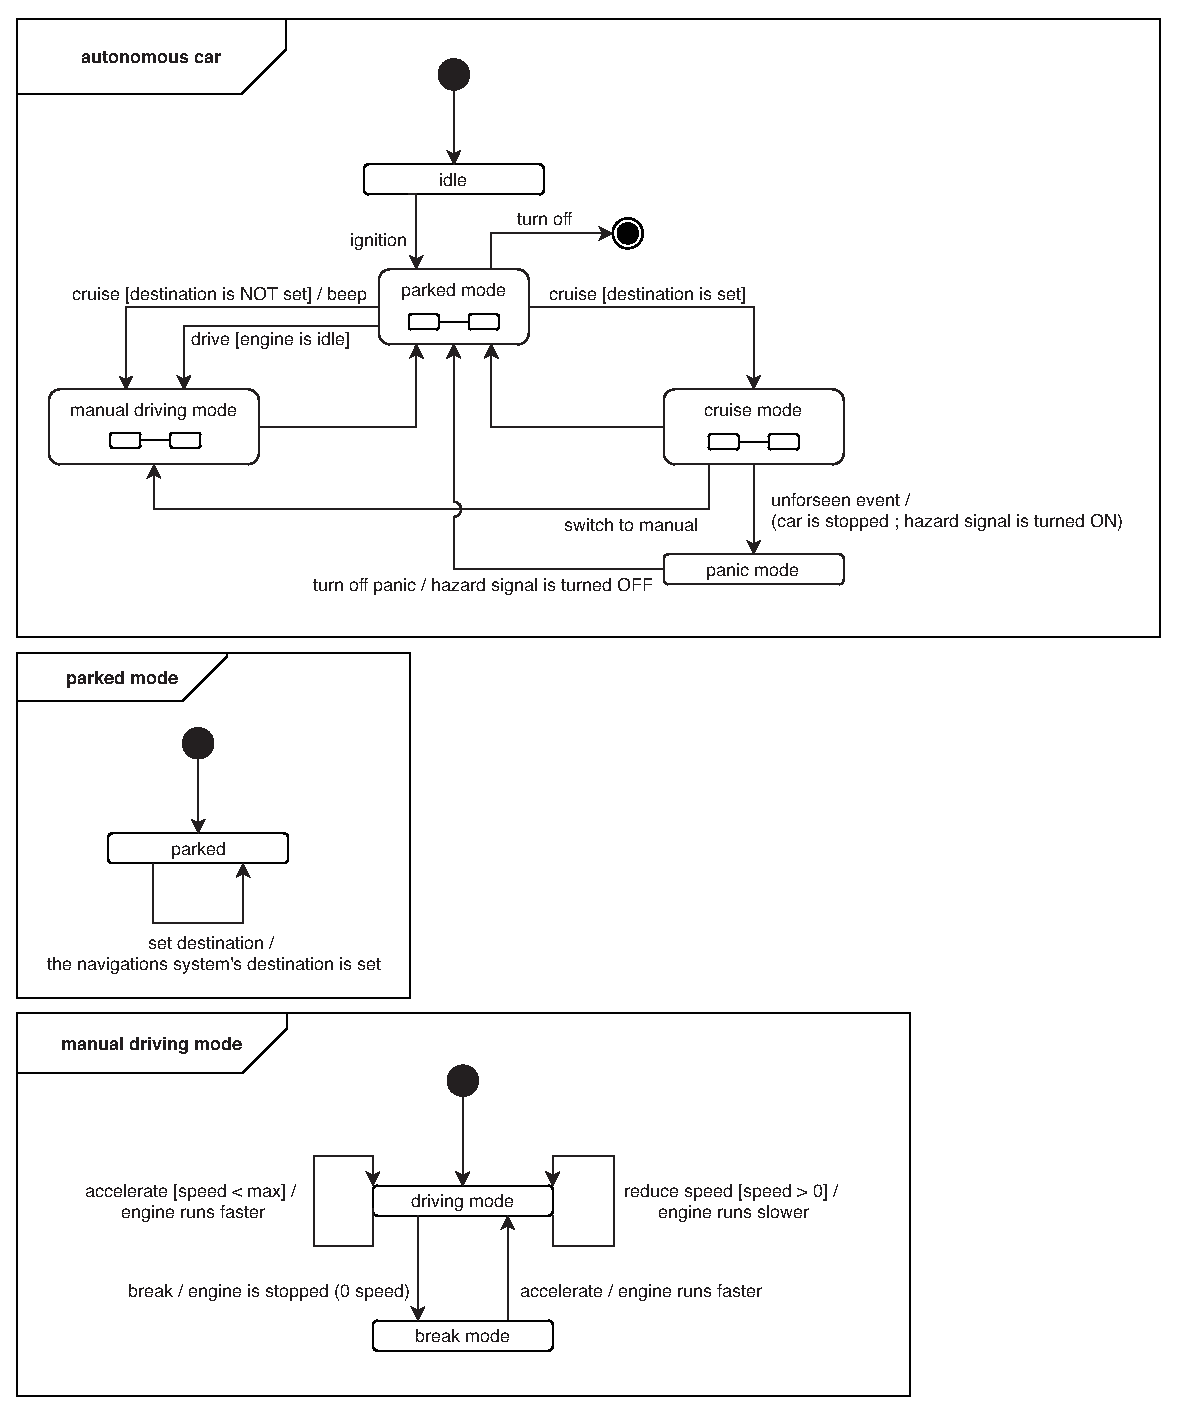
\includegraphics[width=1\textwidth]{./figures/eps/EFSM.eps}
		  \caption{UML state diagram of the autonomous car}
  \label{fig:state-diagram}
\end{figure}
\begin{figure}[h!]
	\centering
		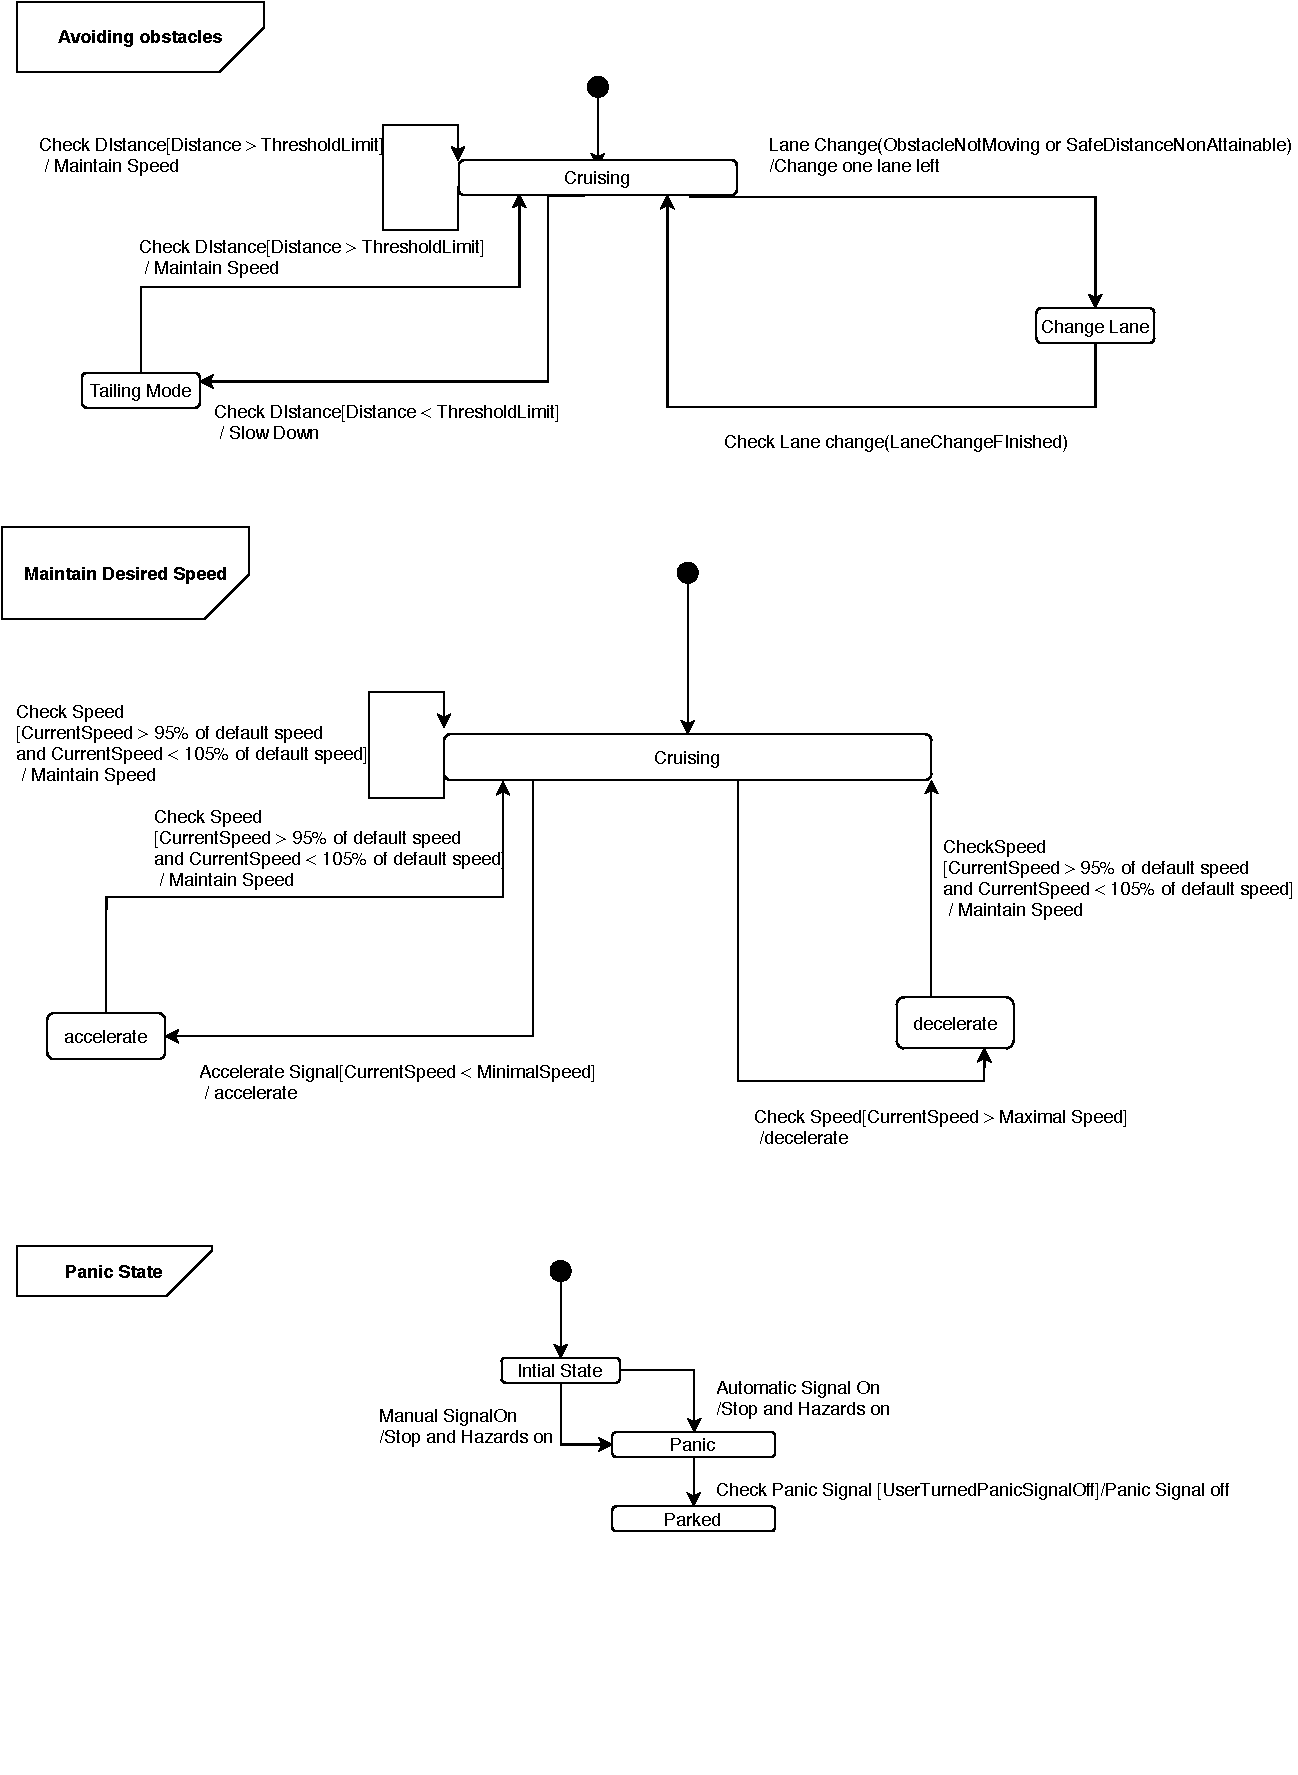
\includegraphics[width=1\textwidth]{./figures/CruiseMode-p2}
		  \caption{UML state diagram of the autonomous car}
  \label{fig:state-diagram}
\end{figure}
\begin{figure}[h!]
	\centering
		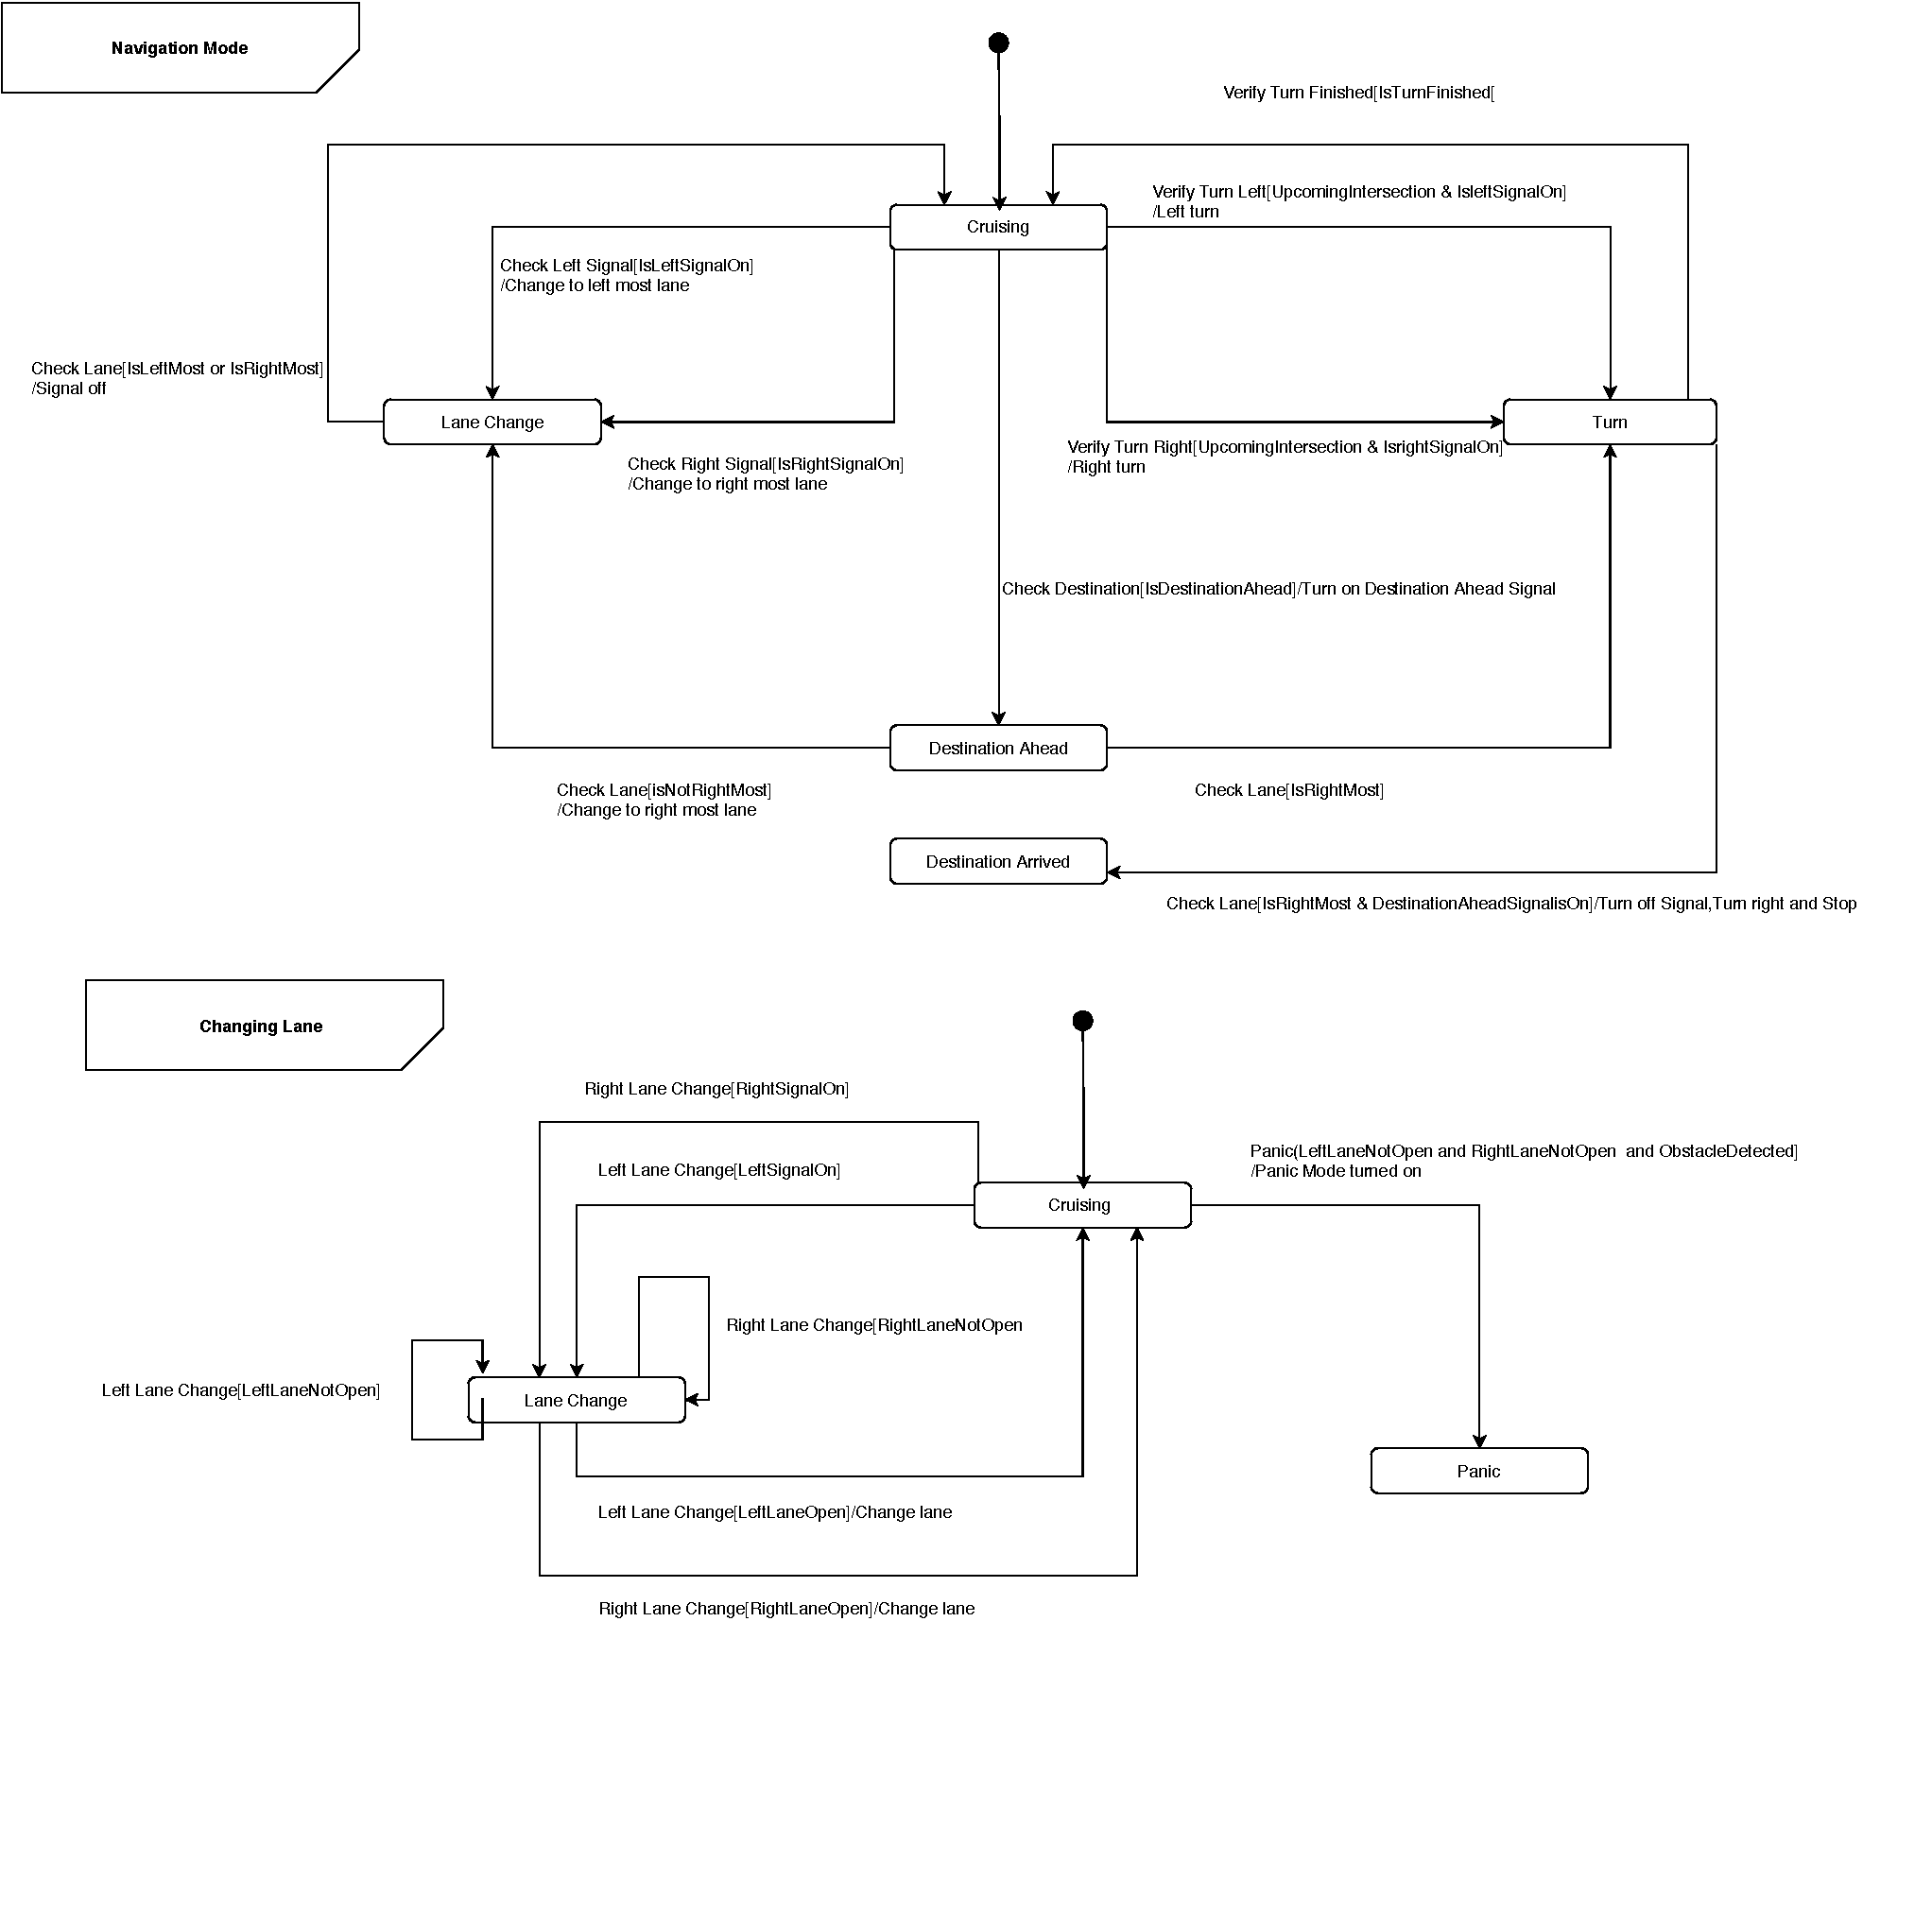
\includegraphics[width=1\textwidth]{./figures/CruiseMode-p3}
		  \caption{UML state diagram of the autonomous car}
  \label{fig:state-diagram}
\end{figure}

\end{spacing}


\end{document}
